\documentclass[8pt]{beamer}
\usepackage[nobglogo]{beamerthemedmi-owled}
\usepackage[utf8x]{inputenc}
\usepackage{default}
\usepackage{url}
\usepackage{verbatim}
\usepackage{graphicx}
\usepackage{mathrsfs}
\usepackage{dl}
\usepackage{mls}
%\usepackage{listings}


\mode<presentation>
{
  \usetheme{dmi-owled}
  %\usetheme{Warsaw}
  % or ...

  \setbeamercovered{transparent}
  % or whatever (possibly just delete it)
}

\title{Web Reasoning 2015/2016\\
Lezione 1}

\author{Cristiano Longo\\ 
{\small{longo@dmi.unict.it}}}



\date{Universit\`a di Catania}
\newcommand{\urlsingle}[1]{{\small {\center {\url{#1}}}}}
\begin{document}
\maketitle
\setcounter{tocdepth}{1}

\section{Introduzione}

\begin{frame}
\frametitle{World Wide Web - nascita}
\begin{quote}
Imagine, then, the references in this document all being associated with 
the network address of the thing to which they referred, so that while 
reading this document you could skip to them with a click of the mouse.
\end{quote}
\vspace{\baselineskip}
\emph{Semantic Web Roadmap}, Tim Berners-Lee, 1989.
\vspace{\baselineskip}

\uncover<2->{
Nel 1993 il CERN rilascer\`a di pubblico dominio i primi software per il
world wide web, tra cui il primo browser chiamato per l'appunto \emph{World
Wide Web}.\footnote{\url{http://home.cern/topics/birth-web}} 
}
\end{frame}

\begin{frame}
\frametitle{World Wide Web - definizione}
\begin{quote}
The World Wide Web (WWW, or simply Web) is an information space in which
the items of interest, referred to as resources, are identified by global
identifiers called Uniform Resource Identifiers (URI).
\end{quote}
\vspace{\baselineskip}
\emph{Architecture of the World Wide Web, Volume
I}\footnote{\url{https://www.w3.org/TR/webarch/}}
\vspace{\baselineskip}

\uncover<2->{
Le prime specifiche rilasciate furono:
\begin{itemize}
  \item Uniform Resource Locators (URLs),
  \item Hypertext Transfer Protocol (HTTP),
  \item Hypertext Markup Language (HTML).
\end{itemize}
}
\end{frame}

\begin{frame}
\frametitle{Limiti del World Wide Web (1/4)}
\begin{quote}
The Web was designed as an information space, with the goal that it should be 
useful not only for human-human communication, but also that machines would be
able to participate and help. One of the major obstacles to this has been the
fact \textbf{that most information on the Web is designed for human consumption}, and 
even if it was derived from a database with well defined meanings (in at least 
some terms) for its columns, that \textbf{the structure of the data is not evident to 
a robot browsing the web.}  
\end{quote}
\vspace{\baselineskip}
\emph{Semantic Web Roadmap}, Tim Berners-Lee, 1998.
\end{frame}

\begin{frame}
\frametitle{Limiti del World Wide Web (2/4)}
Alcuni problemi nell'interpretazione di testi derivano da:
\begin{description}
 \item[Lingue Differenti] e.g. $Parigi$ e $Paris$ possono indicare la stessa citt\`a.
 \item[Omonimie] e.g. esistono svariate citt\`a chiamate 
 \emph{Paris} nel mondo (Arkansas, Idaho, Illinois, Kentucky,
 Maine, Michigan, Missouri, New York, \ldots);
\end{description}
\end{frame}

\begin{frame}
\frametitle{Limiti del World Wide Web (3/4)}

La situazione si complica in presenza di contenuti multimediali.

\begin{figure}
    
\includegraphics[width=250px]{unrecognizable.jpg} 
\end{figure}
\end{frame}

\begin{frame}
\frametitle{Limiti del World Wide Web (4/4)}
Come conseguenza, spesso \`e impossibile eseguire su web ricerce 
\emph{complesse} ottenendo risultati accurati. Ad esempio, cercando sul web
\emph{``Federico II places''} non si ottengono risultati in prima pagina su 
Federico II, ma solo sull'omonima universit\`a:
  
  \begin{small}
    \begin{enumerate}
   \item Universit\`a degli Studi di Napoli "Federico II" | OPEN Places
   \item AOU - Policlinico "Federico II" - Napoli, Italy - Hospital | Facebook
   \item Federico II Ingegneria Via Claudio - College and University | Facebook
   \item MARIA CATERINA FONTE - www.docenti.unina.it
  \end{enumerate}
  \end{small}
\end{frame}

\begin{frame}
\frametitle{Il Web Semantico (1/2)}
\begin{quote}
[\ldots] the Semantic Web approach instead develops languages for expressing
information in a machine processable form. 
\end{quote}
\emph{Semantic Web Roadmap}, Tim Berners-Lee, 1998.

\begin{figure}
    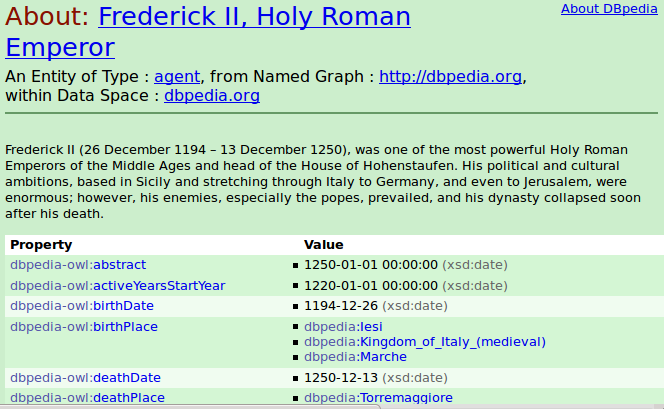
\includegraphics[width=250px]{federicoII_dbpedia.png} 
    \caption{Federico II su dbpedia.org}
\end{figure}
\end{frame}

\begin{frame}
\frametitle{Il Web Semantico - Sintassi}

 Il \emph{Web Semantico} nasce per associare informazioni 
 \emph{strutturate} alle pagine web, che solitamente sono
 composte da testo libero.\footnote{Vedi \emph{Semantic Web Roadmap}, Tim Berners-Lee, 1998.}
 \vspace{\baselineskip}

\uncover<2->{
I \emph{linguaggi di rappresentazione} usati nel Web semantico 
hanno una \emph{sintassi rigorosa}.
\vspace{\baselineskip}
}

\uncover<3->{
Questo rende possibile effettuare interrogazioni complesse 
ottenendo dei risultati precisi anche se a volte parziali:

\begin{center}
Q = “Luoghi di nascita di Federico II e dei suoi parenti stretti” . 
\end{center}
}
\end{frame}

\begin{frame}
\frametitle{Il Web Semantico - Vocabolari}

 L'utilizzo di \emph{vocabolari} condivisi e universalmente riconisciuti,
 spesso dedicati a specifici domini di conoscenza, garantisce
 l'interoperabilit\`a applicativa.
 
\uncover<2->{
 Un esempio di vocabolario \`e \emph{ISA Programme Location Core Vocabulary
 (LOCN).}\footnote{\url{https://www.w3.org/ns/locn}} 
 
 \begin{quote}
 The ISA Programme Location Core Vocabulary provides a minimum set of classes
 and properties for describing any place in terms of its name, address or geometry.
 \end{quote}
}

\uncover<3->{
 \`E possibile realizzare applicativi in grado di trattare informazioni espresse
 con questo vocabolario senza tener conto di chi pubblica le informazioni e
 come.
}
\end{frame}

\begin{frame}
\frametitle{Il Web Semantico - Semantica}

I \emph{linguaggi di rappresentazione} usati nel Web semantico 
sono dotati di una \emph{semantica formale} mutuata dai 
\emph{sistemi di rappresentazione della conoscenza}\footnote{Vedi
Brachman, Schmolze (1985) \emph{An Overview of the KL-ONE Knowledge
Representation System}} e dalle \emph{logiche descrittive}.\footnote{Vedi 
Baader, Calvanese, McGuinness, Nardi, Patel-Schneider \emph{The Description 
Logic Handbook: Theory, Implementation, and Applications, 2nd Edition}.}
\vspace{\baselineskip}

\uncover<2->{
Questo permette di effettuare attivit\`a di \emph{reasoning} (in genere,
inferenze) per
estrarre \emph{conoscenza implicita}.
\vspace{\baselineskip}

Ad esempio, se \`e noto che ``Tutti gli esseri umani sono mortali''
un reasoning engine potr\`a dedurre che ``Socrate \`e mortale''
dal fatto che ``Socrate \`e umano''.
}
\end{frame}

\begin{frame}
\frametitle{Ontologie - definizione}
 I linguaggi di rappresentazione usati nel Web Semantico
 si basano tutti sulla nozione di \emph{ontologia},\footnote{spesso ci si riferisce alle ontologie usando il
termine \emph{dataset}.} mutuata
 dall'ambito dei sistemi di rappresentazione della conoscenza.
\vspace{\baselineskip}

Una \emph{ontologia} \`e una descrizione \emph{parziale} del mondo:
\begin{itemize}
 \item descrive una porzione del mondo, spesso \`e limitata ad un'unico \emph{dominio di conoscenza};
 \item non si assume che i fatti non esplicitamente presenti nell'ontologia siano falsi (\emph{Open World Assumption}).
\end{itemize}
\vspace{\baselineskip}

\uncover<2->{
Essa \`e costituita da un insieme finito di \emph{affermazioni}. Ad esempio le
seguenti affermazioni possono essere espresse in una ontologia:
\begin{itemize}
 \item Tutti gli esseri umani sono mortali;
 \item Socrate \`e mortale;
 \item Alice \`e la madre di Roberto.
\end{itemize}
}
\end{frame}

\begin{frame}
\frametitle{The Semantic Web Stack}
Il Web Semantico \`e un insieme di ontologie presenti sul Web
e rese disponibili usando le tecnologie del Semantic Web Stack.
 
\begin{figure}
    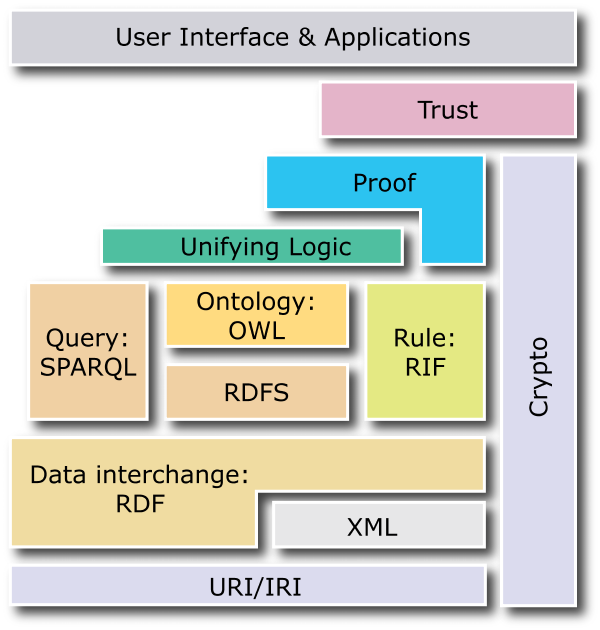
\includegraphics[width=180px]{Semantic_Web_Stack.png}
    \caption{The Semantic Web Stack} 
\end{figure}

\end{frame}

\begin{frame}
\frametitle{Linked Data (1/3)}
\begin{quote}
The Semantic Web is a web of data, in some ways like a global database.
\end{quote}
\small{\emph{Semantic Web Roadmap}, Tim Berners-Lee, 1998.}
\begin{figure}
    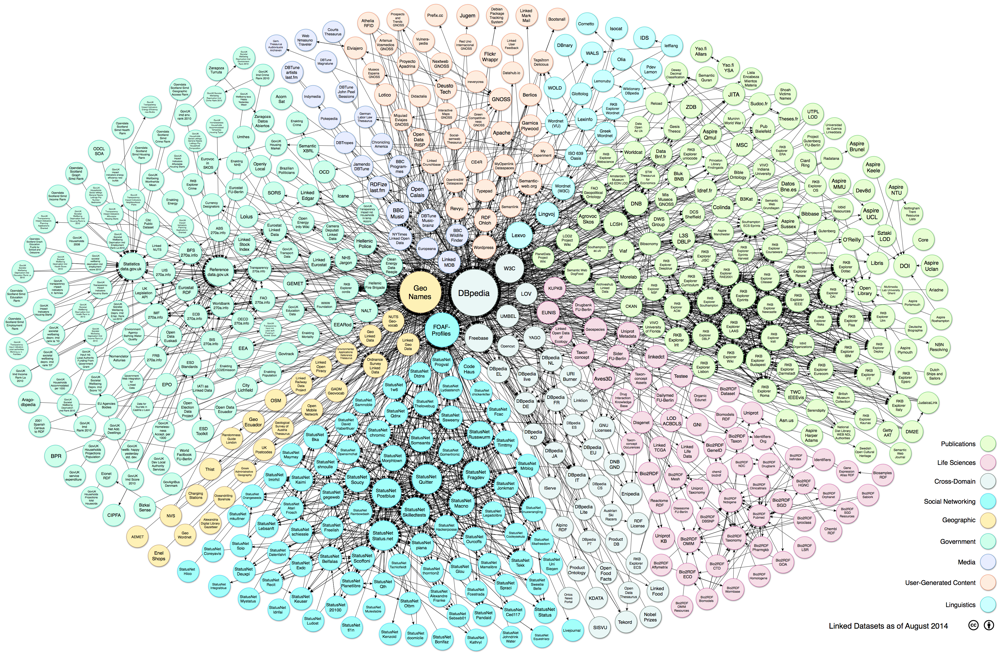
\includegraphics[width=250px]{lod-cloud_colored_1000px.png} 
    \caption{Linked Open Data Cloud}
\end{figure}
\end{frame}

\begin{frame}
\frametitle{Linked Data (2/3)}
Nel \emph{Linked Open Data Cloud} sono presenti 365
\emph{ontologie}(fonte \url{http://stats.lod2.eu/}).
\vspace{\baselineskip}

Alcune di queste sono:
\begin{itemize}
 \item \emph{DBPedia} (\url{dbpedia.org}) corrispondente a \url{wikipedia.org};
 \item \emph{Linked Movie Database} (\url{http://linkedmdb.org/}) controparte sul Web Semantico di \emph{Internet Movie Database} 
 (\url{http://www.imdb.com/});
 \item \emph{Linked GeoData} (\url{http://linkedgeodata.org}) 
  contiene i dati di \emph{OpenStreetMap} (\url{http://www.openstreetmap.org/});
  \item \emph{AGROVOC} (\url{http://aims.fao.org/agrovoc}) \`e l'ontologia della
  FAO (\url{http://fao.org});
  \item \emph{Europeana} (\url{http://pro.europeana.eu/linked-open-data}) contiene dati su beni culturali e tradizioni Europee. 
\end{itemize}
\end{frame}

\begin{frame}
\frametitle{Linked Data (3/3)}
\`E possibile effettuare interrogazioni che coinvolgano diverse
ontologie (anche eterogenee).
\vspace{\baselineskip}

Ad esempio, la seguente query pu\`o essere eseguita
interrogando una ontologia contenente dati storici ed una 
sulle strutture ricettive:


\begin{center}
Q = “Strutture ricettive nei luoghi di nascita di Federico II e dei suoi parenti stretti.”
\end{center}
\end{frame}

\begin{frame}
\frametitle{Argomenti del Corso}

Durante il corso verranno esaminati i principali linguaggi e framework nel
Semantic Web Stack e alcuni strumenti e tecnologie ad essi relativi. Verranno
anche presi in esame alcuni linguaggi generici per la programmazione web.

\begin{itemize}[<+->]
  \item \textbf{Linguaggi del Web Semantico} RDF, RDFS, OWL, SPARQL, \ldots
  \item \textbf{Fondamenti teorici} logica del primo ordine, logiche
  descrittive, \ldots 
  \item \textbf{Linguaggi per il Web} HTML, javascript, PHP, \ldots
  \item \textbf{Strumenti} Prot\'eg\'e, triple stores, reasoner, \ldots 
\end{itemize}

\end{frame}

\section{Ontologie}

\begin{frame}
 \frametitle{Ontologie}
 
 La nozione di \emph{ontologia} usata nel Web Semantico \`e mutuata
 dall'ambito dei sistemi di rappresentazione della conoscenza.
Riportiamo la definizione formale per la sintassi delle ontologie.
\vspace{\baselineskip}

Siano $\CNames$, $\PNames$, $\INames$ tre insiemi infiniti, numerabili e 
a due a due disgiunti di nomi di \emph{classe}, \emph{propriet\`a} e \emph{individuo},
rispettivamente.
\vspace{\baselineskip}

Una \emph{ontologia} \`e un insieme finito di asserzioni dei seguenti tipi:
\[
 \begin{array}{ll}
  \mbox{(Constraints)} & C \Issub D\\
  & P \Issub Q \\
  & \dom(P) \Issub C \\
  & \range(P) \Issub C \\
  &\\
  \mbox{(Class Assertions)} & C(a)\\
  &\\
  \mbox{(Property Assertions)} & a\,P\,b\;(\mbox{equivalente }P(a,b))\\
 \end{array}
\]
dove $C, D \in \CNames$, $P, Q \in \PNames$ e $a, b \in \INames$.
\vspace{\baselineskip}

Si noti che la grammatica per i vincoli ivi riportata \`e \emph{minimale}.
Esistono linguaggi di rappresentazione che permettono di esprimere vincoli
pi\`u complessi.
\end{frame}

\begin{frame}
\frametitle{Ontologie - Sintassi}

 Segue una ontologia presentata a titolo di esempio
\[
\begin{array}{ccl}
 \Ont = & \{ & Woman \Issub Human, \\
 &&Man \Issub Human, \\
 &&Woman \Issub Female, \\
 &&Man \Issub Male, \\
 &&Woman(Alice), \\
 &&Man(Bob),\\
 &&Alice\,relative\,Bob,\\ 
 &&Alice\,child\,Charlie \}
\end{array} 
\]
\end{frame}

\begin{frame}
\frametitle{Ontologie - L'Editor Prot\'eg\'e}

  \emph{Prot\'eg\'e}\footnote{\url{http://protege.stanford.edu/products.php}} 
  \`e una suite per la modellazione di ontologie del Web Semantico, disponibile 
  sia in versione web, che in versione installabile localmente (\emph{Prot\'eg\'e Desktop}).
  \vspace{\baselineskip}

\uncover<2->{
  Permette di definire gerarchie di classi (tab \emph{Classes}) a partire dalla
  classe radice \texttt{Thing}. Per ogni classe \`e possibile definire \emph{label} 
  e \emph{comment} come annotazioni.
  \vspace{\baselineskip}
}

\uncover<3->{
  Analogamente \`e possibile definire gerarchie di propriet\`a (tab \emph{Object Poperties}) 
  a partire dalla propriet\`a radice \texttt{topObjectProperty} e di definire annotazioni
  per le propriet\`a. Inoltre, \`e possibile imporre dei vincoli di dominio e codominio
  per le propriet\`a.
  \vspace{\baselineskip}
}

\uncover<4->{
  Infine \`e possibile definire degli individui (tab \emph{Individuals}) associarli 
  a delle classi di appartenenza e metterli in relazione tra loro attraverso delle
  propriet\`a.
  \vspace{\baselineskip}
}
\end{frame}

\section{Interrogazioni}

\begin{frame}
\frametitle{Interrogazioni}

Il metodo pi\`u immediato per ottenere informazioni da una ontologia \`e il 
\emph{Conjunctive Query Answering}. Consideriamo ad esempio la seguente ontologia:

\begin{tabular}{cc}
\hline
$\begin{array}{cl}
  \Ont  =  &  \{Female(Elise), Female(Alice), Male(Bob), \\
  &\phantom{\{}Male(Charlie), Male(Daniel), \\
  &\phantom{\{}Alice\,childOf\,Elise, Charlie\,childOf\,Elise, \\
  &\phantom{\{}Daniel\,childOf\,Alice, Daniel\,childOf\,Bob, \\
  &\phantom{\{}Francis\,childOf\,Charlie \}
 \end{array}$ & 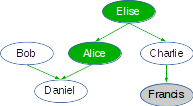
\includegraphics[width=120px]{family.png} \\
\hline
\end{tabular}

Alcune interrogazioni che \`e possibile effettuare con il conjunctive query 
answering sono:
\begin{itemize}
 \item ``Trova tutti gli individui maschi.''
 \item ``Chi sono gli individui con almeno un figlio maschio?''
 \item ``Chi sono i figli di $Alice$?''
 \item ``Chi sono gli individui con almeno un figlio maschio ed una femmina?''
 \item ``Chi sono gli individui maschi con almeno un figlio maschio?''
\end{itemize}
\end{frame}

\begin{frame}
\frametitle{Formule Atomiche}

Per definire in maniera rigorosa le query congiuntive \`e necessario
definire preliminarmente l'insieme delle \emph{formule atomiche}. 
\vspace{\baselineskip}

Sia $\VNames = \{x, y, z, ... \}$ l'insieme infinito, numerabile 
e disgiunto da $\CNames$, $\PNames$ e $\INames$ delle \emph{variabili}.
Le \emph{formule atomiche} sono espressioni dei due seguenti tipi:
\[
 C(\alpha), \quad P(\alpha, \beta)
\]
con $\alpha, \beta \in \INames \cup \VNames$, $C \in \CNames$ e $P \in \PNames$.
\vspace{\baselineskip}

Esempi di formule atomiche sono:
\begin{itemize}
 \item $HumanBeing(x)$,
 \item $x\,childOf\,Alice$,
 \item $Bob\,childOf\,x$,
 \item $x\,childOf\,y$,
 \item $Mortal(Socrate)$,
 \item $Alice\,childOf\,Elise$
\end{itemize}
con $HumanBeing, Mortal \in \CNames$, $childOf \in \PNames$, 
$Alice, Bob, Elise \in \INames$ e $x, y \in \VNames$.
\end{frame}

\begin{frame}
\frametitle{Formule Atomiche Chiuse}
Una formula atomica nella quale non compaiano variabili si dice \emph{chiusa}.
\vspace{\baselineskip}

Negli esempi che seguono sono evidenziate le formule atomiche chiuse:
\begin{itemize}
 \item $HumanBeing(x)$,
 \item $x\,childOf\,Alice$,
 \item $Bob\,childOf\,x$,
 \item $x\,childOf\,y$,
 \item $Mortal(Socrate)$,
 \item $Alice\,childOf\,Elise$
\end{itemize}
con $HumanBeing, Mortal \in \CNames$, $childOf \in \PNames$, 
$Alice, Bob, Elise \in \INames$ e $x, y \in \VNames$.
\vspace{\baselineskip}

\phantom{Le asserzioni presenti nelle ontologie sono formule atomiche chiuse.}
\end{frame}

\begin{frame}
\frametitle{Formule Atomiche Chiuse}
Una formula atomica nella quale non compaiano variabili si dice \emph{chiusa}.
\vspace{\baselineskip}

Negli esempi che seguono sono evidenziate le formule atomiche chiuse:
\begin{itemize}
 \item $HumanBeing(x)$,
 \item $x\,childOf\,Alice$,
 \item $Bob\,childOf\,x$,
 \item $x\,childOf\,y$,
 \item $\mathbf{Mortal(Socrate)}$,
 \item $\mathbf{Alice\,childOf\,Elise}$
\end{itemize}
con $HumanBeing, Mortal \in \CNames$, $childOf \in \PNames$, 
$Alice, Bob, Elise \in \INames$ e $x, y \in \VNames$.
\vspace{\baselineskip}

Le asserzioni presenti nelle ontologie sono formule atomiche chiuse.
\end{frame}

\begin{frame}
\frametitle{Query Congiuntive - }
Una \emph{query congiuntiva} \`e una congiunzione finita di formule atomiche $T_1 \wedge \ldots \wedge T_n$.
\vspace{\baselineskip}

Alcuni esempi di query congiuntive:
\begin{itemize}
 \item ``Trova tutti gli individui maschi.''
 \[
  Male(x)
 \]
 \item ``Chi sono gli individui con almeno un figlio maschio?''
\[
 y\,childOf\,x\,\wedge\,Male(y)  
\]
 \item ``Chi sono i figli di $Alice$?''
\[
 x\,childOf\,Alice
\]
%  \item ``Chi sono gli individui con almeno un figlio maschio ed una femmina?''
% \[
%  y\,childOf\,x\,\wedge\,Male(y)\,\wedge\,z\,childOf\,x\,\wedge\,Female(z)   
% \]
%  \item ``Chi sono gli individui maschi con almeno un figlio maschio?''
% \[
%  Male(x)\,\wedge\,y\,childOf\,x\,\wedge\,Male(y)
% \]
% con $x, y \in \VNames$, $Male, Female \in \CNames$, $childOf \in \PNames$ e $Alice \in \INames$.
 \end{itemize}
con $x, y \in \VNames$, $Male \in \CNames$, $childOf \in \PNames$ e $Alice \in
\INames$.
\end{frame}

\begin{frame}
\frametitle{Sostituzioni (1/2)}

Per definire le \emph{soluzioni} (risposte) delle query congiuntive introduciamo la
nozione di \emph{sostituzione}.
\vspace{\baselineskip}

Una \emph{sostituzione} $\sigma=[x_1 \rightarrow a_1, \ldots, x_n \rightarrow a_n]$
($x_1, \ldots, x_n \in \VNames$, $a_1, \ldots, a_n \in \INames$)
\`e una mappa finita che associa nomi di individui a variabili.
\vspace{\baselineskip}

Sia $T$ una formula atomica e $\sigma=[x_1 \rightarrow a_1, \ldots, x_n \rightarrow a_n]$
una sostituzione. L'\emph{applicazione} $T\sigma$ di $\sigma$ a $T$ \`e la formula atomica 
che si ottiene sostituendo in $T$ ad ogni occorrenza della variabile $x_i$ il
corrispondente nome di individuo $a_i$, per ogni $1\leq i\leq n$.
\vspace{\baselineskip}

Alcuni esempi:
\[
 \begin{array}{lcl}
  Male(x)[x \rightarrow Bob] & = & Male(Bob) \\
  Male(x)[y \rightarrow Bob] & = & \phantom{Male(x)} \\
  (x\,childOf\,y)[x \rightarrow Alice] & = & \phantom{Alice\,childOf\,y} \\
  (x\,childOf\,y)[x \rightarrow Alice, y \rightarrow Elise] & = & \phantom{Alice\,childOf\,Elise}
 \end{array}
\]
con $x,y \in \VNames$, $Male \in \CNames$, $childOf \in \PNames$ e $Alice, Bob, Elise \in \INames$.
\end{frame}

\begin{frame}
\frametitle{Sostituzioni (1/2)}

Per definire le \emph{soluzioni} (risposte) delle query congiuntive introduciamo la
nozione di \emph{sostituzione}.
\vspace{\baselineskip}

Una \emph{sostituzione} $\sigma=[x_1 \rightarrow a_1, \ldots, x_n \rightarrow a_n]$
($x_1, \ldots, x_n \in \VNames$, $a_1, \ldots, a_n \in \INames$)
\`e una mappa finita che associa nomi di individui a variabili.
\vspace{\baselineskip}

Sia $T$ una formula atomica e $\sigma=[x_1 \rightarrow a_1, \ldots, x_n \rightarrow a_n]$
una sostituzione. L'\emph{applicazione} $T\sigma$ di $\sigma$ a $T$ \`e la formula atomica 
che si ottiene sostituendo in $T$ ad ogni occorrenza della variabile $x_i$ il
corrispondente nome di individuo $a_i$, per ogni $1\leq i\leq n$.
\vspace{\baselineskip}

Alcuni esempi:
\[
 \begin{array}{lcl}
  Male(x)[x \rightarrow Bob] & = & Male(Bob) \\
  Male(x)[y \rightarrow Bob] & = & Male(x) \\
  (x\,childOf\,y)[x \rightarrow Alice] & = & \phantom{Alice\,childOf\,y} \\
  (x\,childOf\,y)[x \rightarrow Alice, y \rightarrow Elise] & = & \phantom{Alice\,childOf\,Elise}
 \end{array}
\]
con $x,y \in \VNames$, $Male \in \CNames$, $childOf \in \PNames$ e $Alice, Bob, Elise \in \INames$.
\end{frame}

\begin{frame}
\frametitle{Sostituzioni (1/2)}

Per definire le \emph{soluzioni} (risposte) delle query congiuntive introduciamo la
nozione di \emph{sostituzione}.
\vspace{\baselineskip}

Una \emph{sostituzione} $\sigma=[x_1 \rightarrow a_1, \ldots, x_n \rightarrow a_n]$
($x_1, \ldots, x_n \in \VNames$, $a_1, \ldots, a_n \in \INames$)
\`e una mappa finita che associa nomi di individui a variabili.
\vspace{\baselineskip}

Sia $T$ una formula atomica e $\sigma=[x_1 \rightarrow a_1, \ldots, x_n \rightarrow a_n]$
una sostituzione. L'\emph{applicazione} $T\sigma$ di $\sigma$ a $T$ \`e la formula atomica
che si ottiene sostituendo in $T$ ad ogni occorrenza della variabile $x_i$ il
corrispondente nome di individuo $a_i$, per ogni $1\leq i\leq n$.
\vspace{\baselineskip}

Alcuni esempi:
\[
 \begin{array}{lcl}
  Male(x)[x \rightarrow Bob] & = & Male(Bob) \\
  Male(x)[y \rightarrow Bob] & = & Male(x) \\
  (x\,childOf\,y)[x \rightarrow Alice] & = & Alice\,childOf\,y \\
  (x\,childOf\,y)[x \rightarrow Alice, y \rightarrow Elise] & = & \phantom{Alice\,childOf\,Elise}
 \end{array}
\]
con $x,y \in \VNames$, $Male \in \CNames$, $childOf \in \PNames$ e $Alice, Bob, Elise \in \INames$.
\end{frame}

\begin{frame}
\frametitle{Sostituzioni (1/2)}

Per definire le \emph{soluzioni} (risposte) delle query congiuntive introduciamo la
nozione di \emph{sostituzione}.
\vspace{\baselineskip}

Una \emph{sostituzione} $\sigma=[x_1 \rightarrow a_1, \ldots, x_n \rightarrow a_n]$
($x_1, \ldots, x_n \in \VNames$, $a_1, \ldots, a_n \in \INames$)
\`e una mappa finita che associa nomi di individui a variabili.
\vspace{\baselineskip}

Sia $T$ una formula atomica e $\sigma=[x_1 \rightarrow a_1, \ldots, x_n \rightarrow a_n]$
una sostituzione. L'\emph{applicazione} $T\sigma$ di $\sigma$ a $T$ \`e la formula atomica
che si ottiene sostituendo in $T$ ad ogni occorrenza della variabile $x_i$ il
corrispondente nome di individuo $a_i$, per ogni $1\leq i\leq n$.
\vspace{\baselineskip}

Alcuni esempi:
\[
 \begin{array}{lcl}
  Male(x)[x \rightarrow Bob] & = & Male(Bob) \\
  Male(x)[y \rightarrow Bob] & = & Male(x) \\
  (x\,childOf\,y)[x \rightarrow Alice] & = & Alice\,childOf\,y \\
  (x\,childOf\,y)[x \rightarrow Alice, y \rightarrow Elise] & = & Alice\,childOf\,Elise
 \end{array}
\]
con $x,y \in \VNames$, $Male \in \CNames$, $childOf \in \PNames$ e $Alice, Bob, Elise \in \INames$.
\end{frame}

\begin{frame}
\frametitle{Sostituzioni (2/2)}

L'applicazione di sostituzioni a query congiuntive si definisce come segue.
\vspace{\baselineskip}

Sia $\sigma=[x_1 \rightarrow a_1, \ldots, x_n \rightarrow a_n]$ una sostituzione
e siano $T_1, \ldots, T_m$ formule atomiche. Allora
\[
 (T_1 \wedge \ldots \wedge T_m)\sigma \defAs T_1\sigma \wedge \ldots \wedge T_m\sigma . 
\]
\vspace{\baselineskip}

Alcuni esempi:
\[
 \begin{array}{lcl}
 (y\,childOf\,x\,\wedge\,Male(y))[x \rightarrow Alice] & \defAs & \phantom{y\,childOf\,Alice\,\wedge\,Male(y)}  \\
 (y\,childOf\,x\,\wedge\,Male(y))[x \rightarrow Alice, z \rightarrow Bob] & \defAs & \phantom{y\,childOf\,Alice\,\wedge\,Male(y)}  \\
 (y\,childOf\,x\,\wedge\,Male(y))[x \rightarrow Alice, y \rightarrow Bob] & \defAs & \phantom{Bob\,childOf\,Alice\,\wedge\,Male(Bob)}  \\
 \end{array}
\]
\end{frame}

\begin{frame}
\frametitle{Sostituzioni (2/2)}

L'applicazione di sostituzioni a query congiuntive si definisce come segue.
\vspace{\baselineskip}

Sia $\sigma=[x_1 \rightarrow a_1, \ldots, x_n \rightarrow a_n]$ una sostituzione
e siano $T_1, \ldots, T_m$ formule atomiche. Allora
\[
 (T_1 \wedge \ldots \wedge T_m)\sigma \defAs T_1\sigma \wedge \ldots \wedge T_m\sigma . 
\]
\vspace{\baselineskip}

Alcuni esempi:
\[
 \begin{array}{lcl}
 (y\,childOf\,x\,\wedge\,Male(y))[x \rightarrow Alice] & \defAs & y\,childOf\,Alice\,\wedge\,Male(y)  \\
 (y\,childOf\,x\,\wedge\,Male(y))[x \rightarrow Alice, z \rightarrow Bob] & \defAs & \phantom{y\,childOf\,Alice\,\wedge\,Male(y)}  \\
 (y\,childOf\,x\,\wedge\,Male(y))[x \rightarrow Alice, y \rightarrow Bob] & \defAs & \phantom{Bob\,childOf\,Alice\,\wedge\,Male(Bob)}  \\
 \end{array}
\]
\end{frame}

\begin{frame}
\frametitle{Sostituzioni (2/2)}

L'applicazione di sostituzioni a query congiuntive si definisce come segue.
\vspace{\baselineskip}

Sia $\sigma=[x_1 \rightarrow a_1, \ldots, x_n \rightarrow a_n]$ una sostituzione
e siano $T_1, \ldots, T_m$ formule atomiche. Allora
\[
 (T_1 \wedge \ldots \wedge T_m)\sigma \defAs T_1\sigma \wedge \ldots \wedge T_m\sigma . 
\]
\vspace{\baselineskip}

Alcuni esempi:
\[
 \begin{array}{lcl}
 (y\,childOf\,x\,\wedge\,Male(y))[x \rightarrow Alice] & \defAs & y\,childOf\,Alice\,\wedge\,Male(y)  \\
 (y\,childOf\,x\,\wedge\,Male(y))[x \rightarrow Alice, z \rightarrow Bob] & \defAs & y\,childOf\,Alice\,\wedge\,Male(y)  \\
 (y\,childOf\,x\,\wedge\,Male(y))[x \rightarrow Alice, y \rightarrow Bob] & \defAs & \phantom{Bob\,childOf\,Alice\,\wedge\,Male(Bob)}  \\
 \end{array}
\]
\end{frame}

\begin{frame}
\frametitle{Sostituzioni (2/2)}

L'applicazione di sostituzioni a query congiuntive si definisce come segue.
\vspace{\baselineskip}

Sia $\sigma=[x_1 \rightarrow a_1, \ldots, x_n \rightarrow a_n]$ una sostituzione
e siano $T_1, \ldots, T_m$ formule atomiche. Allora
\[
 (T_1 \wedge \ldots \wedge T_m)\sigma \defAs T_1\sigma \wedge \ldots \wedge T_m\sigma . 
\]
\vspace{\baselineskip}

Alcuni esempi:
\[
 \begin{array}{lcl}
 (y\,childOf\,x\,\wedge\,Male(y))[x \rightarrow Alice] & \defAs & y\,childOf\,Alice\,\wedge\,Male(y)  \\
 (y\,childOf\,x\,\wedge\,Male(y))[x \rightarrow Alice, z \rightarrow Bob] & \defAs & y\,childOf\,Alice\,\wedge\,Male(y)  \\
 (y\,childOf\,x\,\wedge\,Male(y))[x \rightarrow Alice, y \rightarrow Bob] & \defAs & Bob\,childOf\,Alice\,\wedge\,Male(Bob)  \\
 \end{array}
\]
\end{frame}

\begin{frame}
\frametitle{Soluzioni per una Query}
Siano $\sigma=[x_1 \rightarrow a_1, \ldots, x_n \rightarrow a_n]$ una sostituzione,
$Q=T_1 \wedge \ldots \wedge T_m$ una query congiuntiva e $\Ont$ una ontologia.
\vspace{\baselineskip}

$\sigma$ \`e detta essere una \emph{soluzione} per $Q$ rispetto ad $\Ont$ se
e solo se 
\[
	T_i\sigma \in \Ont
\]
per ogni $1\leq i\leq m$. In altre parole, $T_i\sigma$ deve essere in $\Ont$ 
per ogni $T_i$ nella query.
\vspace{\baselineskip}

Consideriamo l'ontologia $\Ont$ e la query $Q$ definite come segue:
\[
\begin{array}{cl}
  \Ont  =  &  \{Female(Elise), Female(Alice), Male(Bob), \\
  &\phantom{\{}Male(Charlie), Male(Daniel), \\
  &\phantom{\{}Alice\,childOf\,Elise, Charlie\,childOf\,Elise, \\
  &\phantom{\{}Daniel\,childOf\,Alice, Daniel\,childOf\,Bob, \\
  &\phantom{\{}Francis\,childOf\,Charlie \}\\
  &\\
  Q = & y\,childOf\,x\,\wedge\,Male(y) .
 \end{array}
\]
Sia $\sigma_1=[x \rightarrow Alice, y \rightarrow Daniel]$. $\sigma_1$ \`e una soluzione per $Q$
rispetto ad $\Ont$?
\end{frame}

\begin{frame}
\frametitle{Soluzioni per una Query - Esempio 1}
Siano $\sigma=[x_1 \rightarrow a_1, \ldots, x_n \rightarrow a_n]$ una sostituzione,
$Q=T_1 \wedge \ldots \wedge T_m$ una query congiuntiva e $\Ont$ una ontologia.
\vspace{\baselineskip}

$\sigma$ \`e detta essere una \emph{soluzione} per $Q$ rispetto ad $\Ont$ se
e solo se $T_1\sigma, \ldots, T_2\sigma$ compaiono in $\Ont$. 
\vspace{\baselineskip}

Consideriamo l'ontologia $\Ont$ e la query $Q$ (``Chi sono gli individui con almeno un figlio maschio?'') definite come segue:
\[
\begin{array}{cl}
  \Ont  =  &  \{Female(Elise), Female(Alice), Male(Bob), \\
  &\phantom{\{}Male(Charlie), \textbf{Male(Daniel)}, \\
  &\phantom{\{}Alice\,childOf\,Elise, Charlie\,childOf\,Elise, \\
  &\phantom{\{}\textbf{Daniel\,childOf\,Alice}, Daniel\,childOf\,Bob, \\
  &\phantom{\{}Francis\,childOf\,Charlie \}\\
  &\\
  Q = & y\,childOf\,x\,\wedge\,Male(y) .
 \end{array}
\]
Sia $\sigma_1=[x \rightarrow Alice, y \rightarrow Daniel]$. $\sigma_1$ \`e una soluzione per $Q$
rispetto ad $\Ont$? \textbf{SI}.
\[
 Q\sigma_1 = Daniel\,childOf\,Alice\,\wedge\,Male(Daniel) .
\]
\end{frame}

\begin{frame}
\frametitle{Soluzioni per una Query - Esempio 2}
Siano $\sigma=[x_1 \rightarrow a_1, \ldots, x_n \rightarrow a_n]$ una sostituzione,
$Q=T_1 \wedge \ldots \wedge T_m$ una query congiuntiva e $\Ont$ una ontologia.
\vspace{\baselineskip}

$\sigma$ \`e detta essere una \emph{soluzione} per $Q$ rispetto ad $\Ont$ se
e solo se $T_1\sigma, \ldots, T_2\sigma$ compaiono in $\Ont$. 
\vspace{\baselineskip}

Consideriamo l'ontologia $\Ont$ e la query $Q$ definite come segue:
\[
\begin{array}{cl}
  \Ont  =  &  \{Female(Elise), Female(Alice), Male(Bob), \\
  &\phantom{\{}Male(Charlie), Male(Daniel), \\
  &\phantom{\{}Alice\,childOf\,Elise, Charlie\,childOf\,Elise, \\
  &\phantom{\{}Daniel\,childOf\,Alice, Daniel\,childOf\,Bob, \\
  &\phantom{\{}Francis\,childOf\,Charlie \}\\
  &\\
  Q = & y\,childOf\,x\,\wedge\,Male(y) .
 \end{array}
\]
Sia $\sigma_2=[x \rightarrow Alice, y \rightarrow Bob]$. $\sigma_2$ \`e una soluzione per $Q$
rispetto ad $\Ont$?
\end{frame}

\begin{frame}
\frametitle{Soluzioni per una Query - Esempio 2}
Siano $\sigma=[x_1 \rightarrow a_1, \ldots, x_n \rightarrow a_n]$ una sostituzione,
$Q=T_1 \wedge \ldots \wedge T_m$ una query congiuntiva e $\Ont$ una ontologia.
\vspace{\baselineskip}

$\sigma$ \`e detta essere una \emph{soluzione} per $Q$ rispetto ad $\Ont$ se
e solo se $T_1\sigma, \ldots, T_2\sigma$ compaiono in $\Ont$. 
\vspace{\baselineskip}

Consideriamo l'ontologia $\Ont$ e la query $Q$ (``Chi sono gli individui con almeno un figlio maschio?'') definite come segue:
\[
\begin{array}{cl}
  \Ont  =  &  \{Female(Elise), Female(Alice), Male(Bob), \\
  &\phantom{\{}Male(Charlie), Male(Daniel), \\
  &\phantom{\{}Alice\,childOf\,Elise, Charlie\,childOf\,Elise, \\
  &\phantom{\{}Daniel\,childOf\,Alice, Daniel\,childOf\,Bob, \\
  &\phantom{\{}Francis\,childOf\,Charlie \}\\
  &\\
  Q = & y\,childOf\,x\,\wedge\,Male(y) .
 \end{array}
\]
Sia $\sigma_2=[x \rightarrow Alice, y \rightarrow Bob]$. $\sigma_2$ \`e una soluzione per $Q$
rispetto ad $\Ont$? \textbf{NO}.
\[
 Q\sigma_2 = \mathbf{Bob\,childOf\,Alice}\,\wedge\,Male(Bob) .
\]
\end{frame}

\begin{frame}
\frametitle{Soluzioni per una Query - Esempio 3}
Siano $\sigma=[x_1 \rightarrow a_1, \ldots, x_n \rightarrow a_n]$ una sostituzione,
$Q=T_1 \wedge \ldots \wedge T_m$ una query congiuntiva e $\Ont$ una ontologia.
\vspace{\baselineskip}

$\sigma$ \`e detta essere una \emph{soluzione} per $Q$ rispetto ad $\Ont$ se
e solo se $T_1\sigma, \ldots, T_2\sigma$ compaiono in $\Ont$. 
\vspace{\baselineskip}

Consideriamo l'ontologia $\Ont$ e la query $Q$ definite come segue:
\[
\begin{array}{cl}
  \Ont  =  &  \{Female(Elise), Female(Alice), Male(Bob), \\
  &\phantom{\{}Male(Charlie), Male(Daniel), \\
  &\phantom{\{}Alice\,childOf\,Elise, Charlie\,childOf\,Elise, \\
  &\phantom{\{}Daniel\,childOf\,Alice, Daniel\,childOf\,Bob, \\
  &\phantom{\{}Francis\,childOf\,Charlie \}\\
  &\\
  Q = & y\,childOf\,x\,\wedge\,Male(y) .
 \end{array}
\]
Sia $\sigma_3=[x \rightarrow Charlie, y \rightarrow Francis]$. $\sigma_3$ \`e una soluzione per $Q$
rispetto ad $\Ont$?
\end{frame}

\begin{frame}
\frametitle{Soluzioni per una Query - Esempio 3}
Siano $\sigma=[x_1 \rightarrow a_1, \ldots, x_n \rightarrow a_n]$ una sostituzione,
$Q=T_1 \wedge \ldots \wedge T_m$ una query congiuntiva e $\Ont$ una ontologia.
\vspace{\baselineskip}

$\sigma$ \`e detta essere una \emph{soluzione} per $Q$ rispetto ad $\Ont$ se
e solo se $T_1\sigma, \ldots, T_2\sigma$ compaiono in $\Ont$. 
\vspace{\baselineskip}

Consideriamo l'ontologia $\Ont$ e la query $Q$ (``Chi sono gli individui con almeno un figlio maschio?'') definite come segue:
\[
\begin{array}{cl}
  \Ont  =  &  \{Female(Elise), Female(Alice), Male(Bob), \\
  &\phantom{\{}Male(Charlie), Male(Daniel), \\
  &\phantom{\{}Alice\,childOf\,Elise, Charlie\,childOf\,Elise, \\
  &\phantom{\{}Daniel\,childOf\,Alice, Daniel\,childOf\,Bob, \\
  &\phantom{\{}Francis\,childOf\,Charlie \}\\
  &\\
  Q = & y\,childOf\,x\,\wedge\,Male(y) .
 \end{array}
\]
Sia $\sigma_3=[x \rightarrow Charlie, y \rightarrow Francis]$. $\sigma_2$ \`e una soluzione per $Q$
rispetto ad $\Ont$? \textbf{NO}.
\[
 Q\sigma_3 = Francis\,childOf\,Charlie\,\wedge\,\mathbf{Male(Francis)} .
\]
\end{frame}

\begin{frame}
\frametitle{Soluzioni per una Query - Esempio 4}
Siano $\sigma=[x_1 \rightarrow a_1, \ldots, x_n \rightarrow a_n]$ una sostituzione,
$Q=T_1 \wedge \ldots \wedge T_m$ una query congiuntiva e $\Ont$ una ontologia.
\vspace{\baselineskip}

$\sigma$ \`e detta essere una \emph{soluzione} per $Q$ rispetto ad $\Ont$ se
e solo se $T_1\sigma, \ldots, T_2\sigma$ compaiono in $\Ont$. 
\vspace{\baselineskip}

Consideriamo l'ontologia $\Ont$ e la query $Q$ definite come segue:
\[
\begin{array}{cl}
  \Ont  =  &  \{Female(Elise), Female(Alice), Male(Bob), \\
  &\phantom{\{}Male(Charlie), Male(Daniel), \\
  &\phantom{\{}Alice\,childOf\,Elise, Charlie\,childOf\,Elise, \\
  &\phantom{\{}Daniel\,childOf\,Alice, Daniel\,childOf\,Bob, \\
  &\phantom{\{}Francis\,childOf\,Charlie \}\\
  &\\
  Q = & y\,childOf\,x\,\wedge\,Male(y) .
 \end{array}
\]
Sia $\sigma_4=[y \rightarrow Daniel]$. $\sigma_4$ \`e una soluzione per $Q$
rispetto ad $\Ont$?
\phantom{Affinch\`e una sostituzione $\sigma$ sia una soluzione per una query $Q$
(a prescindere dall'ontologia) \`e necessario che in $\sigma$ compaiano
tutte le variabili di $Q$.}
\end{frame}

\begin{frame}
\frametitle{Soluzioni per una Query - Esempio 4}
Siano $\sigma=[x_1 \rightarrow a_1, \ldots, x_n \rightarrow a_n]$ una sostituzione,
$Q=T_1 \wedge \ldots \wedge T_m$ una query congiuntiva e $\Ont$ una ontologia.
\vspace{\baselineskip}

$\sigma$ \`e detta essere una \emph{soluzione} per $Q$ rispetto ad $\Ont$ se
e solo se $T_1\sigma, \ldots, T_2\sigma$ compaiono in $\Ont$. 
\vspace{\baselineskip}

Consideriamo l'ontologia $\Ont$ e la query $Q$ (``Chi sono gli individui con almeno un figlio maschio?'') definite come segue:
\[
\begin{array}{cl}
  \Ont  =  &  \{Female(Elise), Female(Alice), Male(Bob), \\
  &\phantom{\{}Male(Charlie), Male(Daniel), \\
  &\phantom{\{}Alice\,childOf\,Elise, Charlie\,childOf\,Elise, \\
  &\phantom{\{}Daniel\,childOf\,Alice, Daniel\,childOf\,Bob, \\
  &\phantom{\{}Francis\,childOf\,Charlie \}\\
  &\\
  Q = & y\,childOf\,x\,\wedge\,Male(y) .
 \end{array}
\]
Sia $\sigma_4=[y \rightarrow Daniel]$. $\sigma_2$ \`e una soluzione per $Q$
rispetto ad $\Ont$? \textbf{NO}.
\[
 Q\sigma_4 = \mathbf{Daniel\,childOf\,x}\,\wedge\,Male(Daniel) .
\]
Affinch\`e una sostituzione $\sigma$ sia una soluzione per una query $Q$
(a prescindere dall'ontologia) \`e necessario che in $\sigma$ compaiano
tutte le variabili di $Q$.
\end{frame}

\begin{frame}
\frametitle{Soluzioni per una Query - Esempio 5}
Siano $\sigma=[x_1 \rightarrow a_1, \ldots, x_n \rightarrow a_n]$ una sostituzione,
$Q=T_1 \wedge \ldots \wedge T_m$ una query congiuntiva e $\Ont$ una ontologia.
\vspace{\baselineskip}

$\sigma$ \`e detta essere una \emph{soluzione} per $Q$ rispetto ad $\Ont$ se
e solo se $T_1\sigma, \ldots, T_2\sigma$ compaiono in $\Ont$. 
\vspace{\baselineskip}

Consideriamo l'ontologia $\Ont$ e la query $Q$ definite come segue:
\[
\begin{array}{cl}
  \Ont  =  &  \{Female(Elise), Female(Alice), Male(Bob), \\
  &\phantom{\{}Male(Charlie), Male(Daniel), \\
  &\phantom{\{}Alice\,childOf\,Elise, Charlie\,childOf\,Elise, \\
  &\phantom{\{}Daniel\,childOf\,Alice, Daniel\,childOf\,Bob, \\
  &\phantom{\{}Francis\,childOf\,Charlie \}\\
  &\\
  Q = & y\,childOf\,x\,\wedge\,Male(y) .
 \end{array}
\]
Sia $\sigma_5=[x \rightarrow Elise, y \rightarrow Charlie, z \rightarrow Francis]$. $\sigma_5$ \`e una soluzione per $Q$
rispetto ad $\Ont$?
\end{frame}

\begin{frame}
\frametitle{Soluzioni per una Query - Esempio 5}
Siano $\sigma=[x_1 \rightarrow a_1, \ldots, x_n \rightarrow a_n]$ una sostituzione,
$Q=T_1 \wedge \ldots \wedge T_m$ una query congiuntiva e $\Ont$ una ontologia.
\vspace{\baselineskip}

$\sigma$ \`e detta essere una \emph{soluzione} per $Q$ rispetto ad $\Ont$ se
e solo se $T_1\sigma, \ldots, T_2\sigma$ compaiono in $\Ont$. 
\vspace{\baselineskip}

Consideriamo l'ontologia $\Ont$ e la query $Q$ (``Chi sono gli individui con almeno un figlio maschio?'') definite come segue:
\[
\begin{array}{cl}
  \Ont  =  &  \{Female(Elise), Female(Alice), Male(Bob), \\
  &\phantom{\{}\mathbf{Male(Charlie)}, Male(Daniel), \\
  &\phantom{\{}Alice\,childOf\,Elise, \mathbf{Charlie\,childOf\,Elise}, \\
  &\phantom{\{}Daniel\,childOf\,Alice, Daniel\,childOf\,Bob, \\
  &\phantom{\{}Francis\,childOf\,Charlie \}\\
  &\\
  Q = & y\,childOf\,x\,\wedge\,Male(y) .
 \end{array}
\]
Sia $\sigma_5=[x \rightarrow Elise, y \rightarrow Charlie, z \rightarrow Francis]$. $\sigma_5$ \`e una soluzione per $Q$
rispetto ad $\Ont$? \textbf{SI}.
\[
 Q\sigma_5 = Charlie\,childOf\,Elise\,\wedge\,Male(Charlie) .
\]
\end{frame}

\begin{frame}
\frametitle{Soluzioni Minimali per una Query}
Siano $\sigma=[x_1 \rightarrow a_1, \ldots, x_n \rightarrow a_n]$ 
una sostituzione, $Q$ una query congiuntiva e $\Ont$ una ontologia.
\vspace{\baselineskip}

$\sigma$ \`e una \emph{soluzione minimale} per $Q$ rispetto a $\Ont$
se e solo se:
\begin{enumerate}
 \item $\sigma$ \`e una soluzione per $Q$ rispetto ad $\Ont$ e inoltre
 \item tutte le variabili $x_1, \ldots, x_n$ che compaiono in $\sigma$
 compaiono anche in $Q$ (criterio di minimalit\`a).
\end{enumerate}
Consideriamo ad esempio
\[
\begin{array}{cl}
  \Ont  =  &  \{Female(Elise), Female(Alice), Male(Bob), \\
  &\phantom{\{}Male(Charlie), Male(Daniel), \\
  &\phantom{\{}Alice\,childOf\,Elise, Charlie\,childOf\,Elise, \\
  &\phantom{\{}Daniel\,childOf\,Alice, Daniel\,childOf\,Bob, \\
  &\phantom{\{}Francis\,childOf\,Charlie \}\\
  &\\
  Q = & y\,childOf\,x\,\wedge\,Male(y) .
 \end{array}
\]
$\sigma_5=[x \rightarrow Elise, y \rightarrow Charlie, z \rightarrow Francis]$ \`e una 
soluzione minimale per $Q$ rispetto a $\Ont$? \phantom{\textbf{NO}.}
\vspace{\baselineskip}

\phantom{$\sigma_6=[x \rightarrow Elise, y \rightarrow Charlie]$ \`e una 
soluzione minimale per $Q$ rispetto a $\Ont$? \textbf{SI}.}
\end{frame}

\begin{frame}
\frametitle{Soluzioni Minimali per una Query}
Siano $\sigma=[x_1 \rightarrow a_1, \ldots, x_n \rightarrow a_n]$ 
una sostituzione, $Q$ una query congiuntiva e $\Ont$ una ontologia.
\vspace{\baselineskip}

$\sigma$ \`e una \emph{soluzione minimale} per $Q$ rispetto a $\Ont$
se e solo se:
\begin{enumerate}
 \item $\sigma$ \`e una soluzione per $Q$ rispetto ad $\Ont$ e inoltre
 \item tutte le variabili $x_1, \ldots, x_n$ che compaiono in $\sigma$
 compaiono anche in $Q$ (criterio di minimalit\`a).
\end{enumerate}
Consideriamo ad esempio
\[
\begin{array}{cl}
  \Ont  =  &  \{Female(Elise), Female(Alice), Male(Bob), \\
  &\phantom{\{}Male(Charlie), Male(Daniel), \\
  &\phantom{\{}Alice\,childOf\,Elise, Charlie\,childOf\,Elise, \\
  &\phantom{\{}Daniel\,childOf\,Alice, Daniel\,childOf\,Bob, \\
  &\phantom{\{}Francis\,childOf\,Charlie \}\\
  &\\
  Q = & y\,childOf\,x\,\wedge\,Male(y) .
 \end{array}
\]
$\sigma_5=[x \rightarrow Elise, y \rightarrow Charlie, \mathbf{z} \rightarrow Francis]$ \`e una 
soluzione minimale per $Q$ rispetto a $\Ont$? \textbf{NO}.
\vspace{\baselineskip}

$\sigma_6=[x \rightarrow Elise, y \rightarrow Charlie]$ \`e una 
soluzione minimale per $Q$ rispetto a $\Ont$? \phantom{\textbf{SI}}.
\end{frame}

\begin{frame}
\frametitle{Soluzioni Minimali per una Query}
Siano $\sigma=[x_1 \rightarrow a_1, \ldots, x_n \rightarrow a_n]$ 
una sostituzione, $Q$ una query congiuntiva e $\Ont$ una ontologia.
\vspace{\baselineskip}

$\sigma$ \`e una \emph{soluzione minimale} per $Q$ rispetto a $\Ont$
se e solo se:
\begin{enumerate}
 \item $\sigma$ \`e una soluzione per $Q$ rispetto ad $\Ont$ e inoltre
 \item tutte le variabili $x_1, \ldots, x_n$ che compaiono in $\sigma$
 compaiono anche in $Q$ (criterio di minimalit\`a).
\end{enumerate}
Consideriamo ad esempio
\[
\begin{array}{cl}
  \Ont  =  &  \{Female(Elise), Female(Alice), Male(Bob), \\
  &\phantom{\{}Male(Charlie), Male(Daniel), \\
  &\phantom{\{}Alice\,childOf\,Elise, Charlie\,childOf\,Elise, \\
  &\phantom{\{}Daniel\,childOf\,Alice, Daniel\,childOf\,Bob, \\
  &\phantom{\{}Francis\,childOf\,Charlie \}\\
  &\\
  Q = & y\,childOf\,x\,\wedge\,Male(y) .
 \end{array}
\]
$\sigma_5=[x \rightarrow Elise, y \rightarrow Charlie, \mathbf{z} \rightarrow Francis]$ \`e una 
soluzione minimale per $Q$ rispetto a $\Ont$? \textbf{NO}.
\vspace{\baselineskip}

$\sigma_6=[x \rightarrow Elise, y \rightarrow Charlie]$ \`e una 
soluzione minimale per $Q$ rispetto a $\Ont$? \textbf{SI}.
\end{frame}

\begin{frame}
\frametitle{Conjunctive Query Answering}
Il problema del \emph{Conjunctive Query Answering} consiste nel trovare
tutte le soluzioni minimali di una query congiuntiva rispetto ad una ontologia.
\vspace{\baselineskip}

Esse sono sempre in numero finito, infatti:
\begin{itemize}
 \item le variabili che compaiono nelle soluzioni sono esattamente quelle che compaiono nella query,
 \item i nomi di individui che compaiono nelle soluzioni sono un sottoinsieme di quelli che compaiono
 nell'ontologia.
\end{itemize}
\end{frame}

\begin{frame}
\frametitle{Conjunctive Query Answering}
Il problema del \emph{Conjunctive Query Answering} consiste nel trovare
tutte le soluzioni minimali di una query congiuntiva rispetto ad una ontologia.
\vspace{\baselineskip}

\begin{center}
Esempio 1:``Trova tutti gli individui maschi.'' 
\end{center}
%\vspace{\baselineskip}

\begin{tabular}{lc}
$\begin{array}{cl}
  \Ont  =  &  \{Female(Elise),  Female(Alice), Male(Bob), \\
  &\phantom{\{}Male(Charlie), Male(Daniel), \\
  &\phantom{\{}Alice\,childOf\,Elise, Charlie\,childOf\,Elise, \\
  &\phantom{\{}Daniel\,childOf\,Alice, Daniel\,childOf\,Bob, \\
  &\phantom{\{}Francis\,childOf\,Charlie \}\\
\end{array}$ &   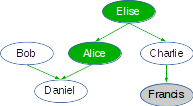
\includegraphics[width=130px]{family.png} \\
 $Q=Male(x)$ &
 $\begin{array}{|c|}
  \hline
  x\\
  \hline
  Bob\\
  Charlie\\
  Daniel\\
  \hline
\end{array}$ \\
\end{tabular}
\end{frame}


\begin{frame}
\frametitle{Conjunctive Query Answering - Esempio 2}
\begin{center}
``Chi sono gli individui con almeno un figlio maschio?'' 
\end{center}

\begin{tabular}{lc}
$\begin{array}{cl}
  \Ont  =  &  \{Female(Elise),  Female(Alice), Male(Bob), \\
  &\phantom{\{}Male(Charlie), Male(Daniel), \\
  &\phantom{\{}Alice\,childOf\,Elise, Charlie\,childOf\,Elise, \\
  &\phantom{\{}Daniel\,childOf\,Alice, Daniel\,childOf\,Bob, \\
  &\phantom{\{}Francis\,childOf\,Charlie \}\\
\end{array}$ &   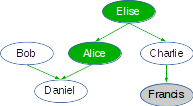
\includegraphics[width=130px]{family.png} \\
 $Q=y\,childOf\,x\,\wedge\,Male(y)$ &
$\begin{array}{|c|c|}
  \hline
  x & y\\
  \hline
  Elise&Charlie\\
  Alice&Daniel\\
  Bob&Daniel\\
  \hline
\end{array}$\\
\end{tabular}
\end{frame}


\begin{frame}
\frametitle{Conjunctive Query Answering - Esempio 3}
\begin{center}
``Chi sono i figli di $Elise$?''
\end{center}

\begin{tabular}{lc}
$\begin{array}{cl}
  \Ont  =  &  \{Female(Elise),  Female(Alice), Male(Bob), \\
  &\phantom{\{}Male(Charlie), Male(Daniel), \\
  &\phantom{\{}Alice\,childOf\,Elise, Charlie\,childOf\,Elise, \\
  &\phantom{\{}Daniel\,childOf\,Alice, Daniel\,childOf\,Bob, \\
  &\phantom{\{}Francis\,childOf\,Charlie \}\\
\end{array}$ & 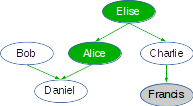
\includegraphics[width=130px]{family.png} \\
$Q=x\,childOf\,Elise$ &
$\begin{array}{|c|}
  \hline
  x\\
  \hline
  \phantom{Alice}\\
  \phantom{Charlie}\\
  \hline
\end{array}$ \\
\end{tabular}
\end{frame}

\begin{frame}
\frametitle{Conjunctive Query Answering - Esempio 3}
\begin{center}
``Chi sono i figli di $Elise$?''
\end{center}

\begin{tabular}{lc}
$\begin{array}{cl}
  \Ont  =  &  \{Female(Elise),  Female(Alice), Male(Bob), \\
  &\phantom{\{}Male(Charlie), Male(Daniel), \\
  &\phantom{\{}Alice\,childOf\,Elise, Charlie\,childOf\,Elise, \\
  &\phantom{\{}Daniel\,childOf\,Alice, Daniel\,childOf\,Bob, \\
  &\phantom{\{}Francis\,childOf\,Charlie \}\\
\end{array}$ & 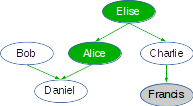
\includegraphics[width=130px]{family.png} \\
$Q=x\,childOf\,Elise$ &
$\begin{array}{|c|}
  \hline
  x\\
  \hline
  Alice\\
  Charlie\\
  \hline
\end{array}$ \\
\end{tabular}
\end{frame}

\begin{frame}
\frametitle{Conjunctive Query Answering - Esempio 4}
\begin{center}
``Chi sono gli individui con almeno un figlio maschio ed una femmina?''
\end{center}

\begin{tabular}{lc}
$\begin{array}{cl}
  \Ont  =  &  \{Female(Elise),  Female(Alice), Male(Bob), \\
  &\phantom{\{}Male(Charlie), Male(Daniel), \\
  &\phantom{\{}Alice\,childOf\,Elise, Charlie\,childOf\,Elise, \\
  &\phantom{\{}Daniel\,childOf\,Alice, Daniel\,childOf\,Bob, \\
  &\phantom{\{}Francis\,childOf\,Charlie \}\\
\end{array}$ & 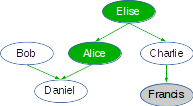
\includegraphics[width=130px]{family.png} \\
$\phantom{Q=y\,childOf\,x\,\wedge\,z\,childOf\,x\,\wedge\,Male(y)\,\wedge\,Female(z)}$ &
$\begin{array}{|c|c|c|}
  \hline
  x&y&z\\
  \hline
  \phantom{Elise}&\phantom{Charlie}&\phantom{Alice}\\
  \hline
\end{array}$ \\
\end{tabular}
\end{frame}

\begin{frame}
\frametitle{Conjunctive Query Answering - Esempio 4}
\begin{center}
``Chi sono gli individui con almeno un figlio maschio ed una femmina?''
\end{center}

\begin{tabular}{lc}
$\begin{array}{cl}
  \Ont  =  &  \{Female(Elise),  Female(Alice), Male(Bob), \\
  &\phantom{\{}Male(Charlie), Male(Daniel), \\
  &\phantom{\{}Alice\,childOf\,Elise, Charlie\,childOf\,Elise, \\
  &\phantom{\{}Daniel\,childOf\,Alice, Daniel\,childOf\,Bob, \\
  &\phantom{\{}Francis\,childOf\,Charlie \}\\
\end{array}$ & 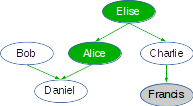
\includegraphics[width=130px]{family.png} \\
$Q=y\,childOf\,x\,\wedge\,z\,childOf\,x\,\wedge\,Male(y)\,\wedge\,Female(z)$ &
$\begin{array}{|c|c|c|}
  \hline
  x&y&z\\
  \hline
  \phantom{Elise}&\phantom{Charlie}&\phantom{Alice}\\
  \hline
\end{array}$ \\
\end{tabular}
\end{frame}

\begin{frame}
\frametitle{Conjunctive Query Answering - Esempio 4}
\begin{center}
``Chi sono gli individui con almeno un figlio maschio ed una femmina?''
\end{center}

\begin{tabular}{lc}
$\begin{array}{cl}
  \Ont  =  &  \{Female(Elise),  Female(Alice), Male(Bob), \\
  &\phantom{\{}Male(Charlie), Male(Daniel), \\
  &\phantom{\{}Alice\,childOf\,Elise, Charlie\,childOf\,Elise, \\
  &\phantom{\{}Daniel\,childOf\,Alice, Daniel\,childOf\,Bob, \\
  &\phantom{\{}Francis\,childOf\,Charlie \}\\
\end{array}$ & 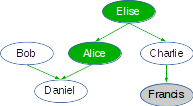
\includegraphics[width=130px]{family.png} \\
$Q=y\,childOf\,x\,\wedge\,z\,childOf\,x\,\wedge\,Male(y)\,\wedge\,Female(z)$ &
$\begin{array}{|c|c|c|}
  \hline
  x&y&z\\
  \hline
  Elise&Charlie&Alice\\
  \hline
\end{array}$ \\
\end{tabular}
\end{frame}


\begin{frame}
\frametitle{Conjunctive Query Answering - Esempio 5}
\begin{center}
``Chi sono gli individui maschi con almeno una figlia femmina?''
\end{center}

\begin{tabular}{lc}
$\begin{array}{cl}
  \Ont  =  &  \{Female(Elise), Female(Alice), Male(Bob), \\
  &\phantom{\{}Male(Charlie), Male(Daniel), \\
  &\phantom{\{}Alice\,childOf\,Elise, Charlie\,childOf\,Elise, \\
  &\phantom{\{}Daniel\,childOf\,Alice, Daniel\,childOf\,Bob, \\
  &\phantom{\{}Francis\,childOf\,Charlie \}\\
\end{array}$ & 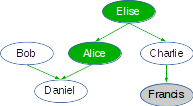
\includegraphics[width=130px]{family.png} \\
$\phantom{Q=Male(x)\,\wedge\,y\,childOf\,x\,\wedge\,Female(y)}$ &
$\begin{array}{|c|c|}
  \hline
  x&y\\
  \hline
  &\\
  &\\
  \hline
\end{array}$\\
\end{tabular}
\end{frame}

\begin{frame}
\frametitle{Conjunctive Query Answering - Esempio 5}
\begin{center}
``Chi sono gli individui maschi con almeno una figlia femmina?''
\end{center}

\begin{tabular}{lc}
$\begin{array}{cl}
  \Ont  =  &  \{Female(Elise), Female(Alice), Male(Bob), \\
  &\phantom{\{}Male(Charlie), Male(Daniel), \\
  &\phantom{\{}Alice\,childOf\,Elise, Charlie\,childOf\,Elise, \\
  &\phantom{\{}Daniel\,childOf\,Alice, Daniel\,childOf\,Bob, \\
  &\phantom{\{}Francis\,childOf\,Charlie \}\\
\end{array}$ & 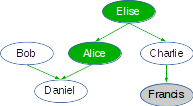
\includegraphics[width=130px]{family.png} \\
$Q=Male(x)\,\wedge\,y\,childOf\,x\,\wedge\,Female(y)$ &
$\begin{array}{|c|c|}
  \hline
  x&y\\
  \hline
  &\\
  &\\
  \hline
\end{array}$\\
\end{tabular}
\end{frame}

\begin{frame}
\frametitle{Conjunctive Query Answering - Esempio 5}
\begin{center}
``Chi sono gli individui maschi con almeno una figlia femmina?''
\end{center}

\begin{tabular}{lc}
$\begin{array}{cl}
  \Ont  =  &  \{Female(Elise), Female(Alice), Male(Bob), \\
  &\phantom{\{}Male(Charlie), Male(Daniel), \\
  &\phantom{\{}Alice\,childOf\,Elise, Charlie\,childOf\,Elise, \\
  &\phantom{\{}Daniel\,childOf\,Alice, Daniel\,childOf\,Bob, \\
  &\phantom{\{}Francis\,childOf\,Charlie \}\\
\end{array}$ & 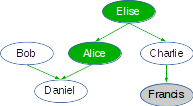
\includegraphics[width=130px]{family.png} \\
$Q=Male(x)\,\wedge\,y\,childOf\,x\,\wedge\,Female(y)$ & Nessuna soluzione\\
\end{tabular}
\end{frame}

\end{document}